% !TEX root=../main.tex
\section{Experiments}\label{sec:experiments}

In this section, we compare the performance of different methods.
We first conduct a simulation study to verify their theoretical reliability.
The effectiveness is further evaluated on a real-world dataset.
All the execution duration is measured on a server with an Intel Xeon E5-2620 CPU @ 2.40GHz (22 cores) and 57GB RAM.
We release our code at \url{https://github.com/NetManAIOps/CIRCA}.
More experiment details are in Appendix~\ref{sec:implementation-details}. 

\subsection{Experimental Setup}

\subsubsection{Hyperparameters}

The shortest sampling interval in our real-world dataset is one minute.
Due to the performance consideration, finer monitoring resolution for each metric is uncommon in OSS.
Thus, different time series will be pre-processed for the same set of timestamps with the same interval of one minute.

% For each fault, $t_{d}$ denotes when the fault is detected \lzy{What is $d$?}.
For each fault, let $t_{d}$ be the \textbf{t}ime a fault is \textbf{d}etected.
We assume that RCA is invoked at $t_{d} + t_{delay}$ to collect necessary information, while it takes data in the period $[t_{d} - t_{ref}, t_{d} + t_{delay}]$ for reference.
The data in $(t_{d} + t_{delay} - t_{test}, t_{d} + t_{delay}]$ are treated as from $P_{\mathbf{m}}$ while $[t_{d} - t_{ref}, t_{d} - t_{test}]$ are taken as fault-free.
By default, we use $t_{delay} = 5$ min, $t_{ref} = 120$ min, and $t_{test} = 10$ min in the experiments.
The effects of different $t_{delay}$ and $t_{ref}$ will be explored in \secref{sec:hyperparameter} with the real-world dataset.
In the rest of this section, we name a fault with its corresponding data in $[t_{d} - t_{ref}, t_{d} + t_{delay}]$ as a \textit{case}.

\subsubsection{Evaluation Metrics}

%We evaluate the performance of a method through the probability that the top-k results recommended by the given method include the root cause metrics, denoted as $AC@k$.
Following existing works~\cite{Wang:2018,Meng:2020,Yu:2021}, we evaluate the performance of a method through the recall with the top-k results, denoted as $AC@k$.
\eqnref{eqn:exp:ac-k} shows the definition of $AC@k$, where $\mathcal{F}$ is a set of faults and $R_{i}(\mathbf{M})$ is the $i$-th result recommended by the method for each fault $\mathbf{M}$.
\eqnref{eqn:exp:ac-k} is slightly different from the evaluation metrics in the previous works~\cite{Wang:2018,Meng:2020,Yu:2021}, ensuring that $AC@k$ is monotonically non-decreasing with $k$.
73\% of developers only consider the top-5 results of a fault localization technique, according to the survey in \cite{Kochhar:2016}.
As a result, we present $AC@k$ for $k \le K = 5$.
Moreover, we show the overall performance by $Avg@K = \frac{1}{K}\sum_{k=1}^{K} AC@k$.
In terms of efficiency, we record analysis duration per fault, denoted as $T$ in the unit of seconds.

\begin{equation}\label{eqn:exp:ac-k}
	AC@k = \frac{1}{|\mathcal{F}|}\sum_{\mathbf{M} \in \mathcal{F}} \frac{|\mathbf{M} \cap \{R_{i}(\mathbf{M}) \mid i = 1, 2, \cdots, k\} |}{\lvert\mathbf{M}\rvert}
\end{equation}

\subsubsection{Baselines}

Each baseline is separated into two steps, namely \textit{graph construction} and \textit{scoring}.
Monitoring metrics will be ranked based on the scores calculated in the final step.
We classify the scoring step in the recent RCA literature for OSS into three groups: DFS-based, random walk-based, and invariant network-based.
In each group, we choose the representative works.
Moreover, we choose the graph construction methods adopted in those works as the baseline ones for the first step.
% We choose baselines for both steps in the recent RCA literature for OSS.

In the graph construction step, the PC algorithm~\cite{Kalisch:2012} is widely used~\cite{Chen:2014,Lin:2018,Wang:2018,Ma:2020}.
We choose Fisher's z-transformation of the partial correlation and $G^{2}$ test as the conditional independence tests for PC, denoted as \textit{PC-gauss} and \textit{PC-gsq}, respectively.
PCMCI~\cite{Runge:2019} adapts PC for time series, based on which \textit{PCTS}~\cite{Meng:2020} transfers the lagged graph into the one among monitoring metrics.
Moreover, the structural graph proposed in this work is denoted as \textit{Structural}.

As for the scoring step, \textit{DFS} traverses the abnormal nodes in the graph, ranking the roots of the sub-graph via anomaly scores~\cite{Chen:2014}.
Its variant \textit{DFS-MS} further ranks candidate metrics according to correlation with the SLI~\cite{Lin:2018}.
Another variant \textit{DFS-MH} traverses the abnormal sub-graph until a node is not correlated with its parents~\cite{Liu:2021}.
The DFS-based methods take the result of anomaly detection as input.
We choose z-score used in \cite{Lin:2018} and SPOT~\cite{Siffer:2017} used in \cite{Meng:2020} as options.
These anomaly detection methods are also taken as baselines\footnote{Anomaly detection and invariant network-based methods will utilize an empty graph with all the available monitoring metrics but no edges.}, denoted as \textit{NSigma} and \textit{SPOT}, respectively.
Another line of works is random walk-based methods.
\textit{RW-Par} calculates the transition probability via partial correlation~\cite{Meng:2020}, while \textit{RW-2} is short for the second-order random walk with Pearson correlation~\cite{Wang:2018}.
\textit{ENMF}\footnote{We take ``ENMF'' from their code to prevent abbreviation duplication between Ranking Causal Anomalies~\cite{Cheng:2016} and Root Cause Analysis.} constructs an invariant network based on the ARX model, explicitly modeling the fault propagation~\cite{Cheng:2016}.
% \footnotemark[ \the\numexpr\value{footnote} - 1\relax]
\textit{CRD} further extends \textit{ENMF} with broken cluster identification~\cite{Ni:2017}.
% \footnote{As the authors' implementation is not available, we implement CRD based on our understanding}

\subsection{Simulation Study}

Three datasets are generated with 50 / 100 / 500 nodes and 100 / 500 / 5,000 edges, respectively, denoted as $\mathcal{D}_{Sim}^{N}$ where $N$ is the number of nodes.
For each dataset, we generate 10 graphs and 100 cases per graph.
Evaluation metrics averaged among the 10 graphs will be presented.
The parameters of baseline methods are selected to achieve the best AC@5 on the first graph in $\mathcal{D}_{Sim}^{50}$.

\subsubsection{Data Generation}

We generate time series based on the Vector Auto-regression model, as shown in \eqnref{eqn:var}.
$\mathbf{x}^{(t)}$ is a column vector of the metrics at time $t$.
$\mathbf{A}$ is the weighted adjacent matrix encoding the CBN.
% $A_{ij} \neq 0$ means the $j$-th metric is a cause of the $i$-th one, where $A_{ij}$ is uniformly sampled from $(-2.0, -0.5) \cup (0.5, 2.0)$ \lzy{why sampling from this range?}, representing the causal effect, \textit{e.g.}, memory usage per request.
$A_{ij} \neq 0$ means the $j$-th metric is a cause of the $i$-th one, where $A_{ij}$ represents the causal effect, \textit{e.g.}, the memory usage per request.
The CBN is enforced to be a connected DAG with only the first node (SLI) having no children.
The item $\beta \mathbf{x}^{(t-1)}$ reflects the auto-regression nature of the time series.
The final item $\mathbf{\epsilon}^{(t)}$ is Gaussian noises, representing the natural fluctuation due to unobserved variables.

\begin{equation}\label{eqn:var}
	\mathbf{x}^{(t)} = \mathbf{A} \mathbf{x}^{(t)} + \beta \mathbf{x}^{(t-1)} + \mathbf{\epsilon}^{(t)}
\end{equation}

To inject a fault $\mathbf{M}$ at time $t$, we first generate the number of root cause metrics $|\mathbf{M}|$.
$|\mathbf{M}| - 1$ follows a Poisson distribution, as it is rare for a fault to affect many metrics directly.
For each $V_{i} \in \mathbf{M}$, the noise item will be altered as $u_{i}^{(t)} = \epsilon_{i}^{(t)} + a_{i} \sigma_{i}$ for 2 timestamps.
The random parameter $a_{i}$ will make the SLI metric abnormal according to the three-sigma rule of thumb.

\subsubsection{Performance Evaluation}

\tableref{tab:performance:sim} summarizes the performance of different methods in three simulation datasets.
The scoring step of each method uses the graph deduced by $\mathbf{A}$ directly, \textit{i.e.}, $X_{j} \in \mathbf{Pa}(X_{i}) \Leftrightarrow \mathbf{A}_{ij} \neq 0$.
We choose the linear regression for RHT.
Moreover, RHT could achieve the best performance in theory if it regards the parents as $\mathbf{Pa}(X_{i}^{(t)}) = \mathbf{Pa}^{(t)}(X_{i}) \cup \left\{X_{i}^{(t-1)}\right\}$.
Such implementation is denoted as \textit{RHT-PG}, where \textit{PG} represents the \textit{perfect graph}.
As the linear relation with the perfect graph performs as the best proxy of $\mathcal{L}_{1}$, we do not consider the descendant adjustment in the simulation study.

RHT-PG approaches the ideal performance, outperforming baseline methods ($p < 0.001$ in t-test for AC@k), which shows the theoretical reliability of our method.
There is a gap between the performance of RHT and RHT-PG, which enlarges as the number of nodes increases.
This phenomenon illustrates the restriction of Corollary~\ref{thm:l2-necessary} that a broken CBN cannot guarantee a correct answer to RCA.
On the other hand, RHT-PG is not perfect yet, which may be the result of statistical errors introduced in hypothesis testing with limited faulty data.

\begin{table*}[tb]
	\caption{
	    Performance of different methods in the simulation study. We put the standard deviation in the parentheses behind each evaluation metric.
	    \textit{RHT-PG} represents \textit{RHT} with the \textit{perfect graph}.
	}\label{tab:performance:sim}
	\begin{tabular}{l ccr ccr ccr}
		\toprule
		\multirow{2}{0.15\columnwidth}{Scoring Method} & \multicolumn{3}{c}{$\mathcal{D}_{Sim}^{50}$} & \multicolumn{3}{c}{$\mathcal{D}_{Sim}^{100}$} & \multicolumn{3}{c}{$\mathcal{D}_{Sim}^{500}$} \\
		& AC@1 & AC@5 & \multirow{1}{0.12\columnwidth}{T (s)} & AC@1 & AC@5 & \multirow{1}{0.12\columnwidth}{T (s)} & AC@1 & AC@5 & \multirow{1}{0.12\columnwidth}{T (s)} \\ 
		\midrule
		NSigma & 0.432(0.05) & 0.733(0.03) & 0.306(0.00) & 0.384(0.05) & 0.613(0.03) & 0.575(0.01) & 0.376(0.04) & 0.579(0.03) & 2.759(0.03) \\
		SPOT & 0.508(0.04) & 0.761(0.03) & 6.601(0.21) & 0.451(0.04) & 0.670(0.03) & 17.365(1.14) & 0.225(0.07) & 0.509(0.07) & 83.465(10.85) \\
		DFS & 0.541(0.04) & 0.682(0.05) & 0.308(0.00) & 0.555(0.03) & 0.653(0.03) & 0.579(0.01) & 0.540(0.03) & 0.611(0.02) & 2.790(0.06) \\
		DFS-MS & 0.515(0.03) & 0.682(0.05) & 0.502(0.00) & 0.517(0.03) & 0.652(0.03) & 0.964(0.01) & 0.191(0.09) & 0.542(0.06) & 4.665(0.06) \\
		DFS-MH & 0.178(0.08) & 0.217(0.09) & 0.501(0.00) & 0.272(0.05) & 0.365(0.05) & 0.969(0.01) & 0.489(0.04) & 0.605(0.03) & 4.735(0.05) \\
		RW-Par & 0.188(0.06) & 0.433(0.07) & 0.714(0.00) & 0.136(0.05) & 0.295(0.07) & 1.761(0.01) & 0.004(0.01) & 0.017(0.02) & 20.246(0.10) \\
		RW-2\footnotemark & 0.188(0.06) & 0.433(0.07) & 0.437(0.00) & 0.136(0.05) & 0.295(0.07) & 1.059(0.01) & 0.004(0.01) & 0.017(0.02) & 10.141(0.11) \\
		ENMF & 0.116(0.03) & 0.278(0.04) & 0.624(0.01) & 0.200(0.03) & 0.336(0.05) & 1.865(0.03) & 0.217(0.04) & 0.354(0.07) & 34.082(0.55) \\
		CRD & 0.074(0.02) & 0.223(0.04) & 4.844(0.03) & 0.013(0.01) & 0.064(0.02) & 6.767(0.10) & 0.003(0.01) & 0.011(0.01) & 46.933(0.74) \\
		RHT & 0.598(0.03) & 0.880(0.02) & 0.338(0.01) & 0.535(0.06) & 0.749(0.06) & 0.658(0.01) & 0.510(0.04) & 0.644(0.04) & 3.326(0.06) \\
		RHT-PG & \textbf{0.615}(0.02) & \textbf{0.952}(0.01) & 0.346(0.00) & \textbf{0.631}(0.02) & \textbf{0.930}(0.01) & 0.665(0.01) & \textbf{0.623}(0.03) & \textbf{0.823}(0.03) & 3.310(0.07) \\
		\midrule
        Ideal & 0.617(0.02) & 0.999(0.00) & & 0.633(0.02) & 0.999(0.00) & & 0.634(0.04) & 1.000(0.00) & \\ 
		\bottomrule
	\end{tabular}
\end{table*}

\footnotetext{RW-2 is degraded to the first-order random walk with its best parameter, hence having the identical performance to RW-Par.\label{footnote:RW-2}}

\subsubsection{Robustness Evaluation}

Faults with the same strength may have different effects on the SLI.
\citeauthor{Yang:2021} name such a phenomenon as the \textit{dependency intensity} in cloud systems, \textit{i.e.}, ``how much the status of the callee service influences the caller service''~\cite{Yang:2021}.
In this simulation study, we further classify faults into three types based on their dependency intensities with the SLI.
We evaluate the performance of RCA methods against faults of each type separately.

\eqnref{eqn:var} can be transformed into $\mathbf{x}^{(t)} = \mathbf{W} (\beta \mathbf{x}^{(t-1)} + \mathbf{\epsilon}^{(t)})$, where $\mathbf{W} = (I - \mathbf{A})^{-1}$.
Notice that $\mathbf{W}$ is well-defined as $\mathbf{A}$ is generated to be a DAG, which does not have full rank.
The element of $\mathbf{W}$ means that $x_{i}$ will increase by $\mathbf{W}_{ij}$ when $x_{j}$ increases by 1.
Denote the standard deviation of $X_{i}$ based on data before fault as $\hat{\sigma}_{i}$.
We classify each fault $\mathbf{M}$ in the simulated datasets into three types:
\begin{description}
	\item[Weak] The root cause metrics deviate from the normal status dramatically to make a slight fluctuation in the SLI (the first node), \textit{i.e.}, $\left(\forall X_{i} \in \mathbf{M}\right) \mathbf{W}_{1i} \hat{\sigma}_{i} / \hat{\sigma}_{1} < 1$;
	\item[Strong] A slight fluctuation in the root cause metrics can change the SLI dramatically, \textit{i.e.}, $\left(\forall X_{i} \in \mathbf{M}\right) \mathbf{W}_{1i} \hat{\sigma}_{i} / \hat{\sigma}_{1} > 1$;
	\item[Mixed] A fault contains metrics with both the above two types or $X_{i}$ with $\mathbf{W}_{1i} \hat{\sigma}_{i} / \hat{\sigma}_{1} = 1$.
\end{description}

\tableref{tab:robustness:sim50} shows the results on $\mathcal{D}_{Sim}^{50}$.
The results on $\mathcal{D}_{Sim}^{100}$ and $\mathcal{D}_{Sim}^{500}$ are omitted since there are only 4 and 5 strong faults in these two datasets, respectively.
RHT and RHT-PG achieve the best results no matter the type of faults, implying that RHT is more robust than baseline methods.
Anomaly detection methods have competitive performance with weak faults.
Their performance drops in strong faults because root cause metrics may be less abnormal than others.
DFS-based methods are sensitive to the results of anomaly detection.
Their performance shares a similar trend with anomaly detection methods, from weak faults to strong ones.

\begin{table}[tb]
	\caption{Robustness evaluation on $\mathcal{D}_{Sim}^{50}$.
	Faults are classified into three types based on their indicators' influence on SLI.}\label{tab:robustness:sim50}
	\setlength{\tabcolsep}{4pt}
	\begin{tabular}{l rr rr rr}
		\toprule
		\multirow{2}{0.12\columnwidth}{Scoring Method} & \multicolumn{2}{c}{Weak (n=916)} & \multicolumn{2}{c}{Mixed (n=64)} & \multicolumn{2}{c}{Strong (n=20)} \\
		& AC@1 & AC@5 & AC@1 & AC@5 & AC@1 & AC@5 \\ 
		\midrule
		NSigma & 0.454 & 0.753 & 0.249 & 0.498 & 0.000 & 0.550 \\
		SPOT & 0.534 & 0.783 & 0.293 & 0.503 & 0.000 & 0.550 \\
		DFS & 0.558 & 0.707 & 0.282 & 0.368 & 0.550 & 0.550 \\
		DFS-MS & 0.531 & 0.707 & 0.277 & 0.368 & 0.550 & 0.550 \\
		DFS-MH & 0.184 & 0.223 & 0.069 & 0.123 & 0.250 & 0.250 \\
		RW-Par & 0.194 & 0.445 & 0.142 & 0.300 & 0.050 & 0.300 \\
		RW-2\textsuperscript{\ref{footnote:RW-2}} & 0.194 & 0.445 & 0.142 & 0.300 & 0.050 & 0.300 \\
		ENMF & 0.111 & 0.269 & 0.124 & 0.321 & 0.300 & 0.550 \\
		CRD & 0.071 & 0.207 & 0.088 & 0.353 & 0.150 & 0.550 \\
		RHT & 0.613 & 0.888 & 0.325 & 0.730 & 0.800 & 1.000 \\
        RHT-PG & \textbf{0.624} & \textbf{0.954} & \textbf{0.358} & \textbf{0.914} & \textbf{1.000} & \textbf{1.000} \\
		\midrule
        Ideal & 0.627 & 1.000 & 0.358 & 0.995 & 1.000 & 1.000 \\ 
		\bottomrule
	\end{tabular}
\end{table}

\subsection{Empirical Study on Oracle Database Data}

We further evaluate different methods in a real-world dataset, denoted as $\mathcal{D}_{O}$.
There are 99 cases in $\mathcal{D}_{O}$.
Each case comes from Oracle databases with high AAS faults in a large banking system.
We choose the parameters of baseline methods for better AC@5.
% We choose the parameters, including the graph construction method, for each scoring method for better AC@5.

\subsubsection{Implementation}

We manually extract the call graph in an Oracle database instance from the official documentation\footnote{Oracle Database Concepts. \url{https://docs.oracle.com/cd/E11882_01/server.112/e40540/}}.
After that, we map 197 monitoring metrics to meta metrics in the skeleton.
The final structural graph contains 2,641 edges.
Oracle database instances may have different sets of metrics.
Therefore, we construct the structural graph for each instance with monitored metrics.

In this empirical study, the ground truth graph is unavailable.
Hence, we compare graph construction methods for each scoring method, choosing the graph with the highest AC@5.
Meanwhile, there is no perfect proxy of $\mathcal{L}_{1}$ (like the CBN and linear relation in the simulation study).
As a result, we fail to include the ideal implementation of RHT (RHT-PG) in the experiment.
We choose the Support Vector Regression (SVR) as the regression method for RHT, which will be discussed in Appendix~\ref{sec:regression-method-selection}.
To alleviate the bias in hypothesis testing, we equip RHT with the descendant adjustment, denoted as \textit{CIRCA}.

\subsubsection{Performance Evaluation}

CIRCA achieves the best results compared with baseline methods, as shown in \tableref{tab:performance:oracle}.
% \lzy{How the combinations of scoring and graph construction methods are selected in this table?}
Random walk-based methods achieve their best performance with PCTS while taking much time to construct the graph.
With the structural graph, DFS-based methods and CIRCA recommend root cause metrics within seconds.
% Anomaly detection alone has competitive performance, which is consistent with the simulation study.

\begin{table}[tb]
	\caption{Performance of different methods on $\mathcal{D}_{O}$}\label{tab:performance:oracle}
	\begin{tabular}{ll rrrr}
		\toprule
		\multirow{2}{0.12\columnwidth}{Scoring Method} & \multirow{2}{0.12\columnwidth}{Graph Method} & \multirow{2}{*}{AC@1} & \multirow{2}{*}{AC@5} & \multirow{2}{*}{Avg@5} & \multirow{2}{0.08\columnwidth}{T (s)} \\
		 & & & & & \\
		\midrule
		NSigma & Empty & 0.323 & 0.662 & 0.525 & 0.472 \\
		SPOT & Empty & 0.152 & 0.419 & 0.296 & 5.027 \\
		DFS & Structural & 0.187 & 0.313 & 0.271 & 0.483 \\
		DFS-MS & Structural & 0.207 & 0.308 & 0.275 & 0.839 \\
		DFS-MH & Structural & 0.268 & 0.439 & 0.372 & 0.844 \\
		RW-Par & PCTS & 0.086 & 0.449 & 0.290 & 24.695 \\
		RW-2\textsuperscript{\ref{footnote:RW-2}} & PCTS & 0.086 & 0.449 & 0.290 & 24.559 \\
		ENMF & Empty & 0.111 & 0.374 & 0.254 & 0.771 \\
		CRD & Empty & 0.035 & 0.313 & 0.165 & 4.787 \\
		CIRCA & Structural & \textbf{0.404} & \textbf{0.763} & \textbf{0.603} & 0.578 \\
		\midrule
        \multicolumn{2}{c}{Ideal} & 0.929 & 1.000 & 0.986 & \\ 
		\bottomrule
	\end{tabular}
\end{table}

We remove components from CIRCA progressively to show their contribution, summarized in \tableref{tab:performance:oracle:components}.
The result illustrates that both regression-based hypothesis testing and descendant adjustment have a positive effect.
\figref{fig:performance:graph-contribution} compares the proposed structural graph with other graph construction baselines.
We exclude anomaly detection and invariant network-based methods from this figure, as they cannot utilize the CBN.
% \lzy{Why only part of scoring methods are presented in this figure?}
Each box in \figref{fig:performance:graph-contribution} presents the distribution of AC@5 for a scoring method with different parameters.
One data point is the best AC@5 from different graph construction parameters with the same scoring ones.
The 3 horizontal lines of each box show 25th, 50th, and 75th percentile, while two whiskers extend to minimum and maximum.
The proposed structural graph improves AC@5 for DFS-based methods and CIRCA, while PCTS fits random walk-based methods better.

\begin{table}[tb]
	\caption{
	Contribution of CIRCA's components on $\mathcal{D}_{O}$ with the structural graph.
	}\label{tab:performance:oracle:components}
	\begin{tabular}{lrrrrr}
		\toprule
		\multirow{2}{0.12\columnwidth}{Scoring Method} & \multirow{2}{*}{AC@1} & \multirow{2}{*}{AC@3} & \multirow{2}{*}{AC@5} & \multirow{2}{*}{Avg@5} & \multirow{2}{0.08\columnwidth}{T (s)} \\
		& & & & & \\
		\midrule
		NSigma & 0.323 & 0.586 & 0.662 & 0.525 &  0.472  \\
		RHT & 0.328 & 0.601 & 0.677 & 0.546 & 0.576 \\
		CIRCA & \textbf{0.404} & \textbf{0.616} & \textbf{0.763} & \textbf{0.603} & 0.578 \\
		\bottomrule
	\end{tabular}
\end{table}

\begin{figure}[tb]
	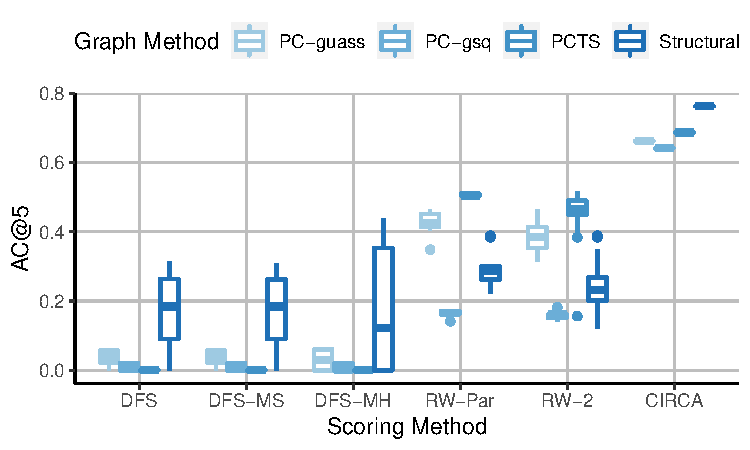
\includegraphics[width=0.83\columnwidth]{img/graph-AC5}
	\caption{AC@5 for different combinations of ranking methods and graph construction ones}\label{fig:performance:graph-contribution}
	\Description{
		This is a box plot for the combination of ranking methods and graph construction methods.
		The boxes for DFS-based methods with PC-gsq or PCTS have AC@5 of zero, while the boxes for DFS-based methods with the proposed structural graph are higher than those with PC-gauss.
		As for random walk-based ranking methods, the boxes with PCTS are higher than other graph construction methods.
	}
\end{figure}

\subsubsection{Case Study}

\figref{fig:performance:case} presents a failure, where ``log file sync'' (LFS) is the root cause metric labeled by the database administrators (DBAs).
A poor understanding of $\mathcal{L}_{1}$ puzzles RCA methods.
On the one hand, DFS fails to stop at LFS and continues to check ``execution per second'' (EPS), missing the desired answer.
No baseline method recommends LFS in the top-5 results, except NSigma, ENMF, and CRD.
% \lzy{How does other baselines perform on this cases? For example, RW?}
On the other hand, CIRCA assigns a high anomaly score for AAS after revising it from 532.4 (given by NSigma) to 480.2 with regression.

% CIRCA scores each metric separately to prevent missing the desired answer \lzy{I did not get how it helps}.
DFS-based methods will drop descendants once meeting an abnormal metric.
In contrast, CIRCA scores each metric separately, preventing missing answers like DFS-based methods.
Moreover, CIRCA adjusts the anomaly score of LFS with that of the average time of ``log file parallel write'' (LFPW), \textit{i.e.}, $s_{LFS}^{\prime} = 7028.6$.
% showing the preference for the former \lzy{Maybe add more description about the anomaly score adjustion}.
This technique helps CIRCA rank LFS ahead of the other metrics.

\begin{figure}[tb]
	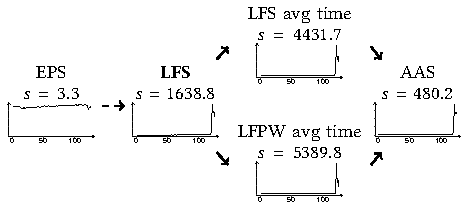
\includegraphics{img/case}
	\caption{
	    Part of an Oracle database failure, where LFS is the root cause metric labeled by the DBAs.
	   % Below each metric name is the anomaly score calculated by \eqnref{eqn:anomaly-score} and the time series at the same period.
	    Below each metric name is the score calculated by \eqnref{eqn:anomaly-score} and the time series at the same period.
	    Time (horizontal axis) is shown in minutes.
	   % We hide the value (vertical axis) due to the confidentiality policy of our partner company.
	}\label{fig:performance:case}
	\Description{
	    This figure shows part of an Oracle database failure.
	    LFS is the root cause metric.
	    One of its parent, EPS, has an anomaly score slightly larger than 3.
	    On the other hand, the anomaly scores of LFS and its descendants are higher than 480.
	}
\end{figure}

\subsubsection{Lessons Learned}

CIRCA outperforms baseline methods on $\mathcal{D}_{O}$, consistent with the simulation study.
\tableref{tab:performance:oracle:components} and \figref{fig:performance:graph-contribution} further illustrate that each of the 3 proposed techniques has a positive effect.

Though RCA is a difficult task related to Layer 2 of the causal ladder (Corollary~\ref{thm:l2-necessary}), the knowledge of Layer 1 ($\mathcal{L}_{1}$) is incomplete.
We illustrate the negative effect through a case study.
We believe that further advancement in the future has to handle this obstacle explicitly.
At present, we prefer CIRCA to pure RHT if deployed.
Meanwhile, the effectiveness of the descendant adjustment has to be verified on more real-world datasets.

% \subsection{Case Study on Bank Information System Data}

% \textbf{TODO:}
% \cite{Cheng:2016} evaluates their method on a Bank Information System (BIS) dataset, which is in their repository.

\subsection{Discussion}

\subsubsection{Hyperparameter Sensitivity}\label{sec:hyperparameter}

% \figref{fig:param-sensitivity} shows the performance of each method with different $t_{delay}$ and $t_{ref}$.
\figref{fig:param-sensitivity} compares RCA methods with different $t_{delay}$ and $t_{ref}$.
CIRCA has stable performance with these two hyperparameters, outperforming baseline methods.

\begin{figure}[tb]
	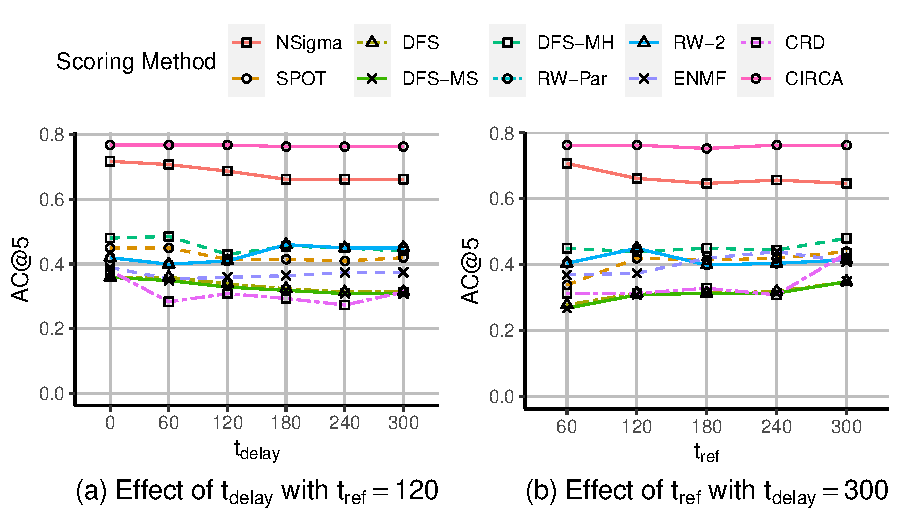
\includegraphics[width=0.9\columnwidth]{img/param-sensitivity}
	\caption{Performance with various hyperparameters on $\mathcal{D}_{O}$}\label{fig:param-sensitivity}
	\Description{
		There are two line charts, showing the performance of baseline methods with different hyperparameters.
		The left one fixes $t_{ref} = 120$, varying $t_delay$, while the right one fixes $t_{delay} = 300$, varying $t_ref$.
	}
\end{figure}

\subsubsection{Performance of Existing Methods}

% DFS-based methods are sensitive to anomaly detection.
% If we cannot reach the SLI from the root cause metrics along with abnormal nodes, a DFS-based method cannot locate the root cause.

RW-Par and RW-2 represent the scoring methods of MicroCause~\cite{Meng:2020} and CloudRanger~\cite{Wang:2018}, respectively.
However, RW-Par (RW-2) fails to achieve the performance in the corresponding paper.
MicroCause utilizes metric priority provided by operators, which is unavailable for RW-Par.
On the other hand, CloudRanger achieves its best result with a sampling interval of 5 seconds.
% Though it is feasible with trace data, it is impractical for massive metrics.
The coarse monitoring frequency of $\mathcal{D}_{O}$ may explain the poor performance of RW-2.

As stated by Corollary~\ref{thm:l2-necessary}, knowledge of Layer 2 (such as $\mathbf{Pa}$) is necessary for RCA.
The invariant network-based methods utilize the observation data only (Layer 1).
Their unsatisfying performance illustrates the restriction of CHT~\cite{Bareinboim:2022}.

\subsubsection{Feasibility}

\noindent
\textbf{Graph Construction.}
% \paragraph{Graph Construction}
The construction of the proposed structural graph requires system architecture and a mapping from monitoring metrics to the targets to be monitored.
The former is usually in the form of documentation.
We argue that a metric is neither insightful nor actionable unless operators understand its underlying meaning.
Operators need to classify each distinct metrics only once to obtain the mapping.
The mapping can be shared among similar instances of the same type (like Oracle database instances).

\noindent
\textbf{Scalability.}
% \paragraph{Scalability}
As shown in \tableref{tab:performance:sim}, RHT's time cost grows around linearly with the size of the dataset.
% \lzy{It seems CIRCA costs too much time on a large-scale system (tens of thousands of instances)}
Moreover, the design of CIRCA supports horizontal scalability to handle large-scale systems via adding computing resources, as each metric is scored separately.
We plan to train the regression models offline to speed up online analysis.
Mature parallel programming frameworks, such as Apache Spark, may further help accelerate CIRCA.
